%\chapter{Preliminaries}
\chapter{実験1}

\section{目的}

    実験1では、輝度を一定とした複数の色の刺激に対して知覚される光沢感を被験者ごとに測定を行う。
    色度ごとの光沢感を定量化することで、光沢感に色度情報が寄与しているかどうかを明らかにすることを目的とする。
    また、以下に記す仮説が成立するかどうかを明らかにする。

\section{仮説}

    上記の通り、物体の鏡面反射成分の輝度が光沢感知覚に寄与していることは既知である。
    しかし、明確に輝度が寄与しているか知覚的な明るさが寄与しているかは不明である。
    輝度と知覚的な明るさに違いをもたらす現象としてHelmholtz-Kohlrausch効果(以下H-K効果)が知られている。
    これは、同一の輝度を有する色でも彩度が高いほど明るく感じられ、特に青・紫・赤紫・赤などの色相を有する色により明るく見えるという効果である。

    実験1を行う前に、拡散反射成分と鏡面反射成分の知覚的な明るさのコントラストが主に光沢感に寄与しているという仮定を立てた。
    反射成分のうち、拡散反射成分は鏡面反射成分に比べて低輝度である。
    そこで反射成分を拡散反射成分と鏡面反射成分に分け、拡散反射成分のみに輝度を変えずに着色処理を行う。
    H-K効果による明るさ感の増幅が顕著な色度では、他色度に比べて相対的に明るさのコントラストが大きく減少するため、光沢感が小さいということになる。
    すなわち、H-K効果の明るさの増幅度合いと光沢感には負の相関が現れると予想される。

\section{実験方法}
    \subsection{実験環境}

        \begin{figure}
            \centering
            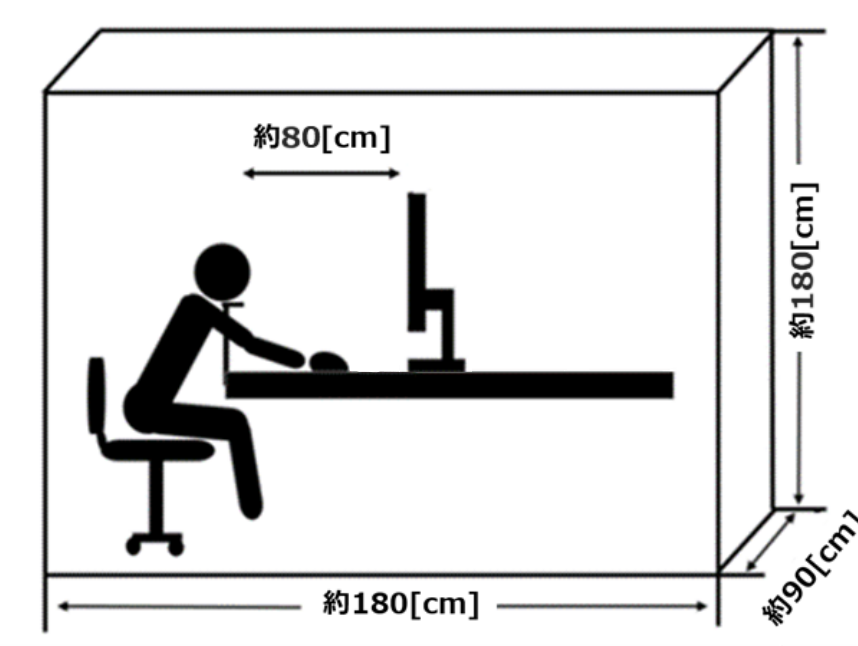
\includegraphics[width=10.0cm]{./img/darkroom_p.png}
            \caption{実験環境概略図}
            \label{darkroom}
        \end{figure}

        図???に実験環境の概略図を示す。
        暗幕で覆われた簡易的な暗室内に刺激呈示用液晶ディスプレイ (EIZO, 解像度 1920 ピクセル✕ 1200 ピクセル, リフレッシュレート 60 Hz) を設置し実験を行った。
        また、刺激の輝度と色度を正確に投影するために分光反射輝度計( Cambridge Research Systems 社 SpectroCAL ) によりモニタの分光分布を、色彩輝度計( Cambridge Research Systems 社 ColorCAL2 )によりモニタのガンマ特性を測定した。
        これにより、所望のCIE XYZ三刺激値をモニタに呈示することが可能となった。
        
        実験はすべてPC ( DELL 社 Vostro 13 5000, OS: Ubuntu 18.04.3 LTS) で統制され、MathWorks MATLAB と Psychtoolbox3 を用いてプログラムを作成・実行することでディスプレイの刺激呈示と被験者応答を管理した。
        実験中、被験者の頭部はディスプレイから 80 cm の距離に顎台により固定され、両眼自然視でディスプレイを観察した。
        被験者はトラックボールマウスを使用して応答した。

    \subsection{実験刺激}

        \begin{figure}
            \centering
            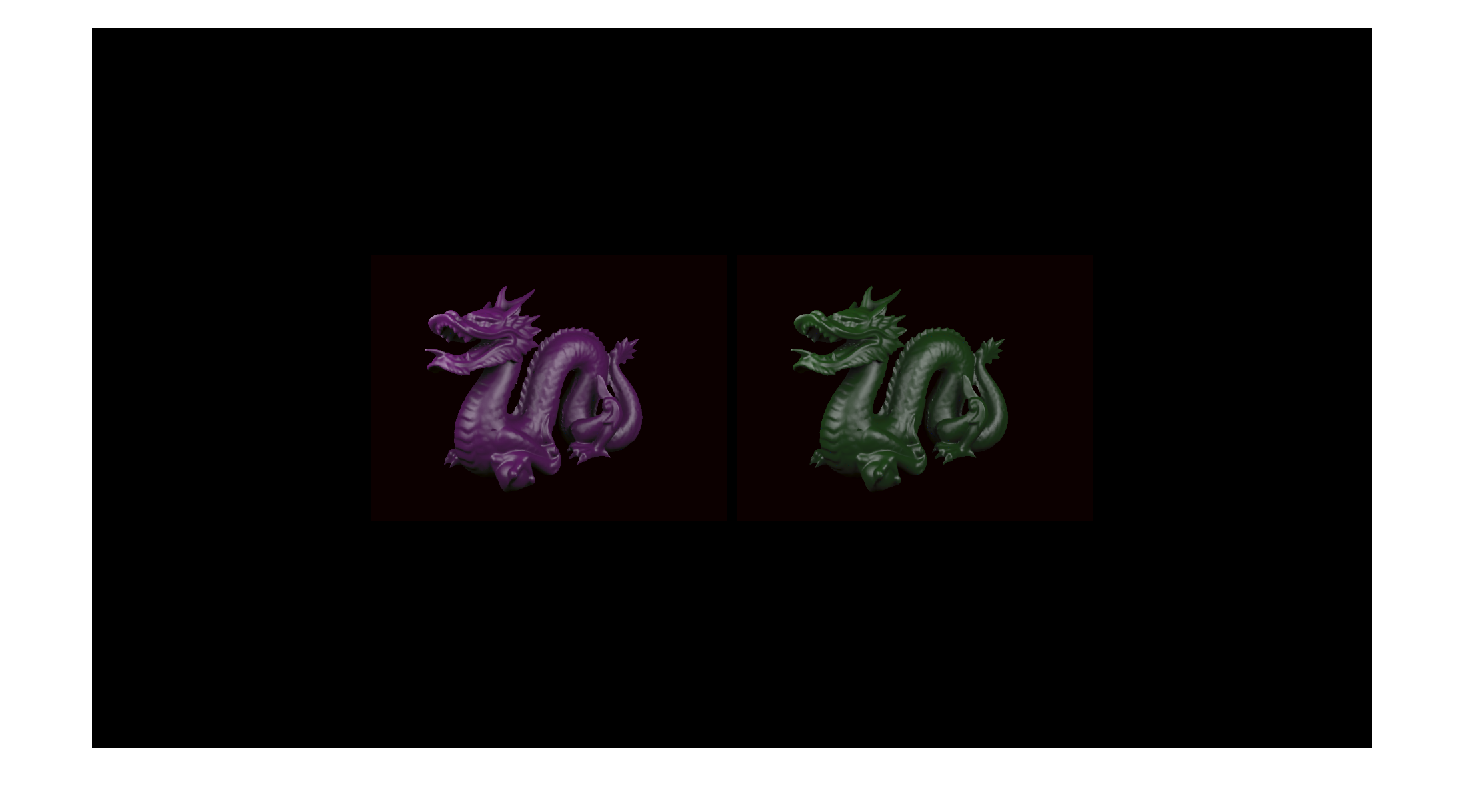
\includegraphics[width=14.0cm]{./img/ex1_stimuli.png}
            \caption{1試行に呈示される実験刺激の例}
            \label{darkroom}
        \end{figure}

        図 ??? に実験1で使用する刺激を示す。
        刺激は黒背景上の縦 6.42 deg, 横 17.35 deg の範囲の左右に呈示される二枚のコンピュータグラフィックス画像であった。
        これらの画像はモニタ中央を挟んで対称な位置に提示された。
        また、各画像はコンピュータグラフィックスソフトウェアを用いたレンダリングと、MATLAB上での簡易的な画像処理を用いた着色の二つの工程を経て作られた。
        以下に、これらの工程の詳細を記す。

        \subsubsection{レンダリング}

            実験に用いた刺激の元となる無彩色刺激は RenderToolbox4 によって, レンダラーを Mitsuba として作成された。
            この際の照明環境はCIE標準光源D65であり、物体の分光反射特性は全波長にわたり同じ値であった。
            物体形状として、Stanford Dragon と Stanford Bunny [todo: 引用情報] を使用し、照明環境も含めた環境のジオメトリはBlender 2.79により設定した。
            一方、表面反射特性は RenderToolbox4 と Mitsuba により設定し、その反射モデルとして Ward モデルを用いた。
            この際、拡散反射成分と鏡面反射成分の色度を別々に操作するため、これらの反射成分は独立にレンダリングした。
            このレンダリングにおけるパラメータを表 ??? に実験1で使用する刺激を示す。

            \begin{table}
                \centering
                \caption{レンダリング時のパラメータ}
                \begin{tabular}{|l||c|c|c|} \hline
                                           & SpecularReflectance & DiffuseReflectance & Roughness \\ \hline \hline
                    拡散反射成分           & 0                   & 0.1                & 0.2 \\ \hline
                    鏡面反射成分           & 0.9                 & 0                  & 0.2 \\ \hline
                \end{tabular}
            \end{table}
        
        \subsubsection{着色}

            レンダリングされた画像は上述したとおりD65の色度を持つ画像であったが、その画像に対して色条件を設定するために色度を付与した。
            その方法はSD着色とD着色の2種類であった。
            SD着色では、拡散反射成分と鏡面反射成分の両方に同じ色度を設定し、それらのCIE XYZ値を加算して作成した。
            D着色では、拡散反射成分にのみ着色を行い、XYZ値を加算して作成した。
            この着色処理において、Mitsubaによってレンダリングされた画像のXYZ三刺激値をu’v’Y色空間に変換し、u’v’色度図上で行われた。
            その色度は全部で9種類である。
            そのうち1種類はD65の色度であり、これを白色点とする。
            その他の8種類の色度は、白色点を中心とし、u’v’色度図上の0°から45°間隔となる8方向にある色度であった。
            本論文では、これらの9色度をそれぞれgray, red, orange, yellow, green, blue-green, cyan, blue, magentaと呼ぶことにする。

            レンダリングされた画像(以下raw画像)は高輝度域を含む画像であった。
            モニタが表示可能な色域は輝度によって異なり、特にモニタが表示できる最大・最小輝度付近におけるu'v'色度図の領域は非常に小さい。
            すなわち、この画像に対して着色処理を行った場合、鏡面反射成分に十分な彩度の色度を付与することができないため、SD着色条件とD着色条件を十分に差別化することができない。
            このため、線形トーンマッピングによって画像の最高輝度を下げた。

            また、モニタが表示可能な色域は色相によっても異なる。レンダリングされた画像にモニタの色域外の色度を付与しないように、画像の輝度を対数尺度を用いて200段階に標本化し、そのそれぞれの輝度に対して9種類の色度の白色点から最大距離となる点を計測した。


    \subsection{実験手続き}

        \begin{figure}
            \centering
            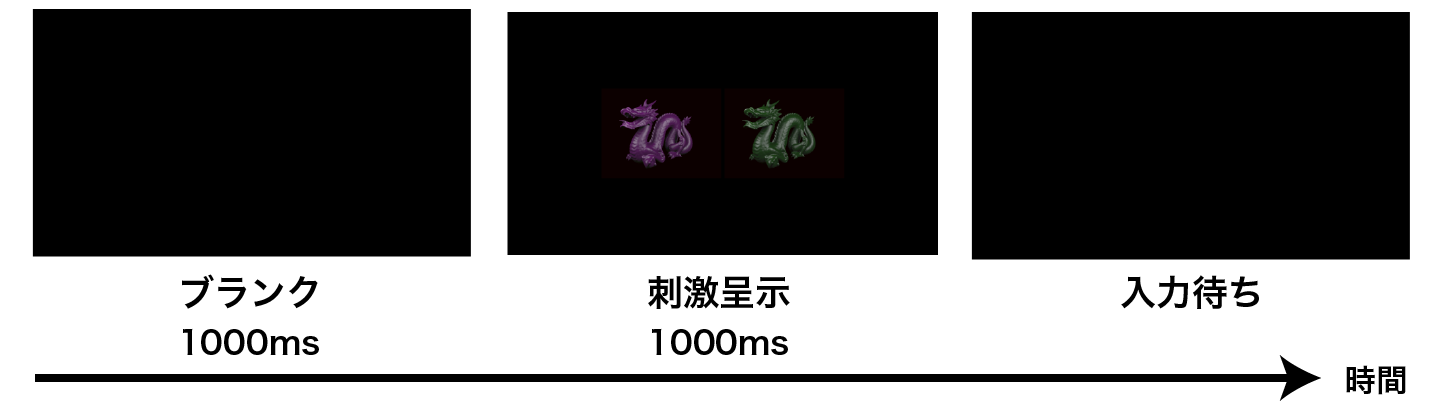
\includegraphics[width=14.0cm]{./img/ex1_procedure.png}
            \caption{実験1の1試行の流れ}
            \label{ex1_procedure}
        \end{figure}

        実験1はサーストンの一対比較法を用いて行われた。
        実験1の1試行の流れを図 ??? に示す。各試行はまず黒背景のみからなるブランク画面の1000msの呈示から始まる。
        その後、刺激対が1000msの間呈示され、さらに、色順応を避けるために黒背景のみからなる入力待ち画面に移行した。
        刺激対の呈示中または入力待ち画面で、被験者は右画像と左画像のうちどちらからより光沢感を強く知覚するかを、マウスの左クリックまたは右クリックにより応答した。
        このとき次の試行のブランク画面に移行した。

        各セッションは 2 着色条件 ✕ 物体形状 2 種類 ✕ 色の組み合わせ 36 通り = 144 試行からなり、各被験者は全体で4セッションの実験を行った。
        各セッションの 144 試行で使われる刺激対は全てランダムな順序で選ばれた。
        1セッションに要する時間はおよそ8分であり、2セッション目と3セッション目の間に一度だけ休憩をとった。



\section{実験結果}
    \subsection{解析方法}

    \subsection{考察}
        
        \begin{figure}
            \centering
            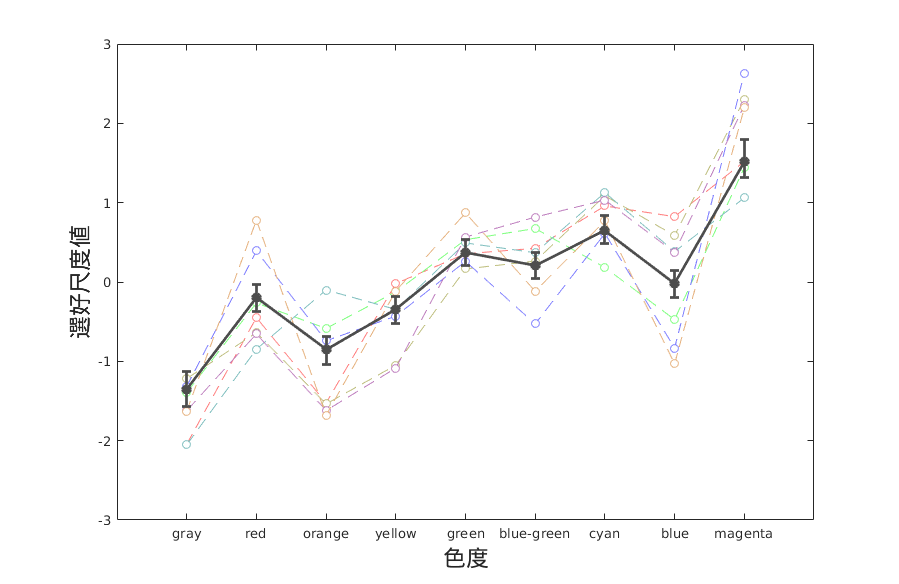
\includegraphics[width=14.0cm]{./img/ex1_res_DSD.png}
            \caption{Dragon:SD着色条件における選好尺度値}
            \label{ex1_DSD}
        \end{figure}

        \begin{figure}
            \centering
            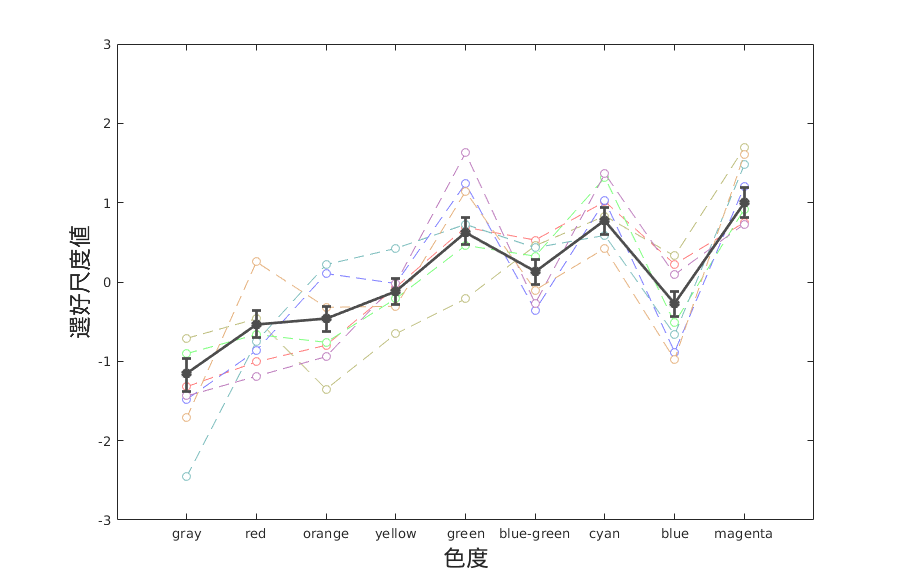
\includegraphics[width=14.0cm]{./img/ex1_res_BSD.png}
            \caption{Bunny:SD着色条件における選好尺度値}
            \label{ex1_BSD}
        \end{figure}

        \begin{figure}
            \centering
            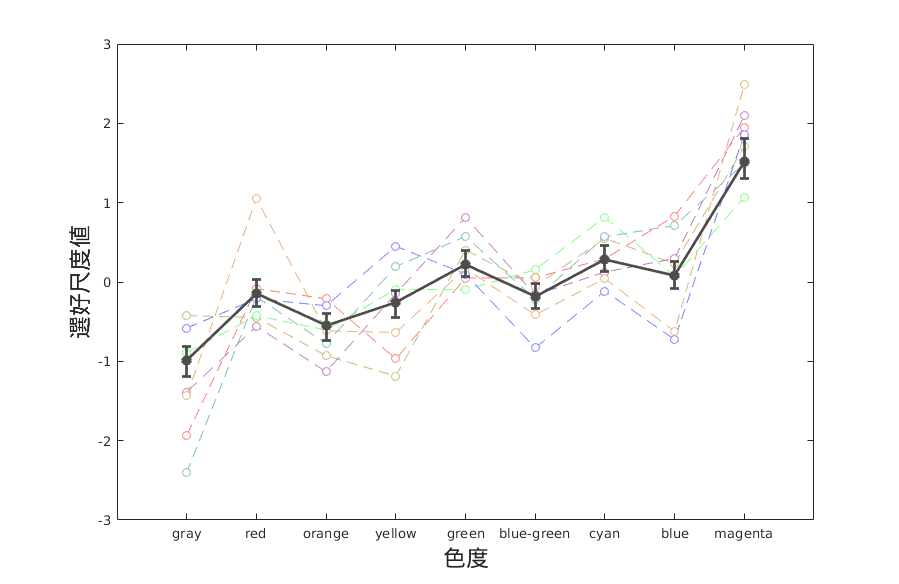
\includegraphics[width=14.0cm]{./img/ex1_res_DD.png}
            \caption{Dragon:D着色条件における選好尺度値}
            \label{ex1_DD}
        \end{figure}

        \begin{figure}
            \centering
            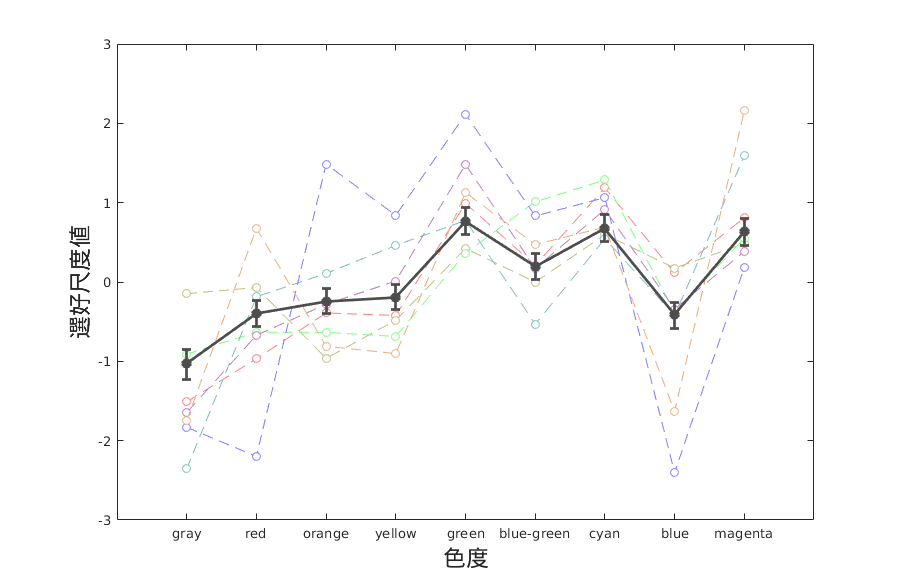
\includegraphics[width=14.0cm]{./img/ex1_res_BD.png}
            \caption{Bunny:SD着色条件における選好尺度値}
            \label{ex1_BD}
        \end{figure}

        物体形状や着色条件に関わらず、すべての条件において色度により光沢感が異なることがわかる。
        特にBunny:D着色条件を除いてmagentaの光沢感が極めて高く、次いでgreen,cyanの光沢感が高いという結果となった。
        Dragon:SD着色, Bunny:SD着色, Dragon:D着色の3条件で似た傾向が見られたが、Bunny:D着色条件ではblueとmagentaの光沢感が相対的に低い値であった。

        仮説通りであれば、D着色条件においてredやmagentaの色度における光沢感は他の色度に比べて低いはずであるが、Dragon,Bunnyの両方でそのような傾向は見られない。
        このため、光沢感が拡散反射と鏡面反射の知覚的な明るさのコントラストによって主に決まっているという訳ではないと言える。

        ここで、SD着色条件とD着色条件で傾向に大きな違いが見られないこと、magentaの光沢感が極端に大きいことに着目する。
        明るさのコントラストではなく、刺激全体を通して感じられる明るさが光沢感に寄与しているのではないかと考え、次の実験2を行った。
